% !TeX root = ../main.tex

\chapter{Methods and algorithms}
\label{chapt:methods}

\section{Discretisation of the Yukawa theory}
\label{sec:lattice_discretisation}
In order to make the theory suitable for a numerical simulation on a computer, the continuum formulation of the Yukawa model, which has been introduced in section \ref{sec:Yukawa_theory}, has to be discretised. Here we provided a sketch of a discretisation procedure, and we refer to other resources \cite{rothe_LGT,gattringer_LQCD,creutz_2023,Montvay1994QuantumLattice} for further details. \\~\\
For what concerns the bosonic part of the action, a discretisation can be done straightforwardly with the following replacements
\begin{equation*}
    \begin{aligned}
        \int d^x \quad &\to \quad a^2 \sum_x, \\
        \partial^2_t + \partial^2_x = \frac{\partial^2}{\partial t^2} + \frac{\partial^2}{\partial x_1^2} \quad &\to \quad \sum_\mu \left[\frac{\delta_{m,n+\mu} + \delta_{m,n-\mu} - 2 \delta_{m,n}}{a^2}\right],
    \end{aligned}
\end{equation*}
which yields to the lattice action
\begin{equation*}
        \begin{aligned} 
        		S_\phi [\phi] 	&=  a^2 \left( \frac{1}{2} \, \sum_{m,n} \phi_m \, K_{mn} \, \phi_n + \frac{\lambda}{4!} \, \sum_n \phi_n^4 \right)\\
        					&=  \frac{1}{2} \, \sum_{m,n} \hat{\phi}_m \, \widehat{K}_{mn} \, \hat{\phi}_n + \frac{\hat{\lambda}}{4!} \, \sum_n \hat{\phi}_n^4,
	\end{aligned}
\end{equation*}
where we expressed everything in dimensionless quantities
\begin{equation}
    \begin{aligned}
        \hat m_\phi^2 &= a^2 \, m_\phi^2, \\
        \hat \lambda &= a^{2} \, \lambda, \\
        \widehat{K}_{mn} &= a^2 K_{mn}.
    \end{aligned}
    \label{eq:couplings_redefitinion}
\end{equation}
The operator components $\widehat{K}_{mn}$ are the discretised version of \eqref{eq:definition_kinetic_terms_continuum_position}
\begin{equation}
    \widehat{K}_{mn} = - \sum_\mu \left[\delta_{m,n+\mu} + \delta_{m,n-\mu} - 2 \, \delta_{m,n}\right] + \hat{m}_\phi^2 \, \delta_{mn} 
    \label{eq:discretised_kinetic_op_bosons}
\end{equation}
and its representation in momentum space is
\begin{equation*}
	\begin{aligned}
		\widehat{K}_{p, q} & =\sum_{n, m} e^{i p n} \, \widehat{K}_{n m} \, e^{-i q m} \\
		& =\sum_{n, m} e^{i p n}\left(-\sum_\mu\left[\delta_{m,m+\mu}+\delta_{m,m-\mu}-2 \delta_{m, n}\right] + \hat{m}_\phi^2 \, \delta_{mn}\right) e^{-i q m} \\
		& =\sum_{n} e^{i(p-q) n}\left[\hat{m}_\phi^2+2\sum_\mu \left(1-\cos \left(q_\mu\right)\right)\right] \\
		& = \left[\hat{m}_\phi^2 + \sum_\mu 4 \sin ^2\left(\frac{p_\mu}{2}\right) \right] \, \delta(p-q) .
	\end{aligned}
\end{equation*}
For what concerns the fermionic action, a na\"ive discretisation is not sufficient, due to the well known doubling problem \cite{rothe_LGT,Montvay1994QuantumLattice}. In this work Wilson fermions \cite{wilson_lqcd} are employed as a way to fix such issue. Details of this formulation are explained in Appendix \ref{chap:AppendixB}. Here, only the final discretised action is reported, which reads
\begin{equation}
		S_\psi\left[\psihat, \psibarhat \right] + S_\text{int}\left[\phihat, \psihat, \psibarhat \right] = \sum_{f=1}^{N_f}\hat{\bar{\psi}}_m^{(f)} \, \widehat{D}_{mn} \, \hat{\psi}_n^{(f)},
\end{equation}
with $\psi_n$ beeing a two-component spinor, and $\widehat{D}_{m,n}$ the Wilson-Dirac operator \textcolor{blue}{(can I include $g\phi $ in the definition of $D$?)} defined as 
\begin{equation}
    \begin{aligned}
    \widehat{D}_{m, n} = &- \left(\frac{\Gamma_{+\hat 0}}{2} \, \delta_{m, m+\hat 0} +\frac{\Gamma_{-\hat 0}}{2} \, \delta_{m, m-\hat 0} + \frac{\Gamma_{+\hat 1}}{2} \, \delta_{m, m+\hat 1} + \frac{\Gamma_{- \hat 1}}{2} \, \delta_{m, m-\hat 1}\right)  \\
     &+ \left(2ar + \hat m + \hat g \phi\right) \, \delta_{s,s'} \, \delta_{m,n}. \\
    \end{aligned}
    \label{eq:wilson-dirac_operator}
\end{equation}
Note that the interaction term $g\, \bar\psi\phi\psi$ has been included in the definition of $D$. \\
The Wilson projectors $\Gamma_{\pm \hat \mu}$ are defined as
\begin{equation*}
    \Gamma_{\pm \hat \mu} = ar \, \mathds{1}_s \mp \gamma_\mu.
\end{equation*}
Since $r \in [0,1]$ is a free parameter, in this work we set $r=1$, if not otherwise specified. \\
In summary the discretised action for the Yukawa model is 
\begin{equation*}
    S\left[\phihat, \psihat, \psibarhat \right] = \sum_{m,n} \, \hat{\phi}_m \, \widehat{K}_{m,n} \, \hat{\phi}_n + \frac{\hat{\lambda}}{4!} \, \hat{\phi}_m^{\,4} \, \delta_{m,n} + \sum_{f=1}^{N_f}\psibarhat_m^{(f)} \, \widehat{D}_{mn} \psihat_n^{(f)},
\end{equation*}
with $\widehat{K}_{mn}, \widehat{D}_{mn}$ given respectively by \eqref{eq:discretised_kinetic_op_bosons} and \eqref{eq:wilson-dirac_operator}. \\
For later reference, we also report the discretised version of the effective action \eqref{eq:effective_action_no_fermions}
\begin{equation}
	\begin{aligned}
		S_\text{eff}[\hat\phi] 	&= S_\phi[\hat\phi] - N_f \trover{n,s} \log \widehat{D} \\
							&= \sum_{m,n} \, \hat{\phi}_m \, \widehat{K}_{m,n} \, \hat{\phi}_n + \frac{\hat{\lambda}}{4!} \, \hat{\phi}_m^{\,4} \, \delta_{m,n} - N_f \trover{n,s} \log \widehat{D}_{nn}.
	\end{aligned}
	\label{eq:discretised_effective_action}
\end{equation}
The full discrete path-integral reads \textcolor{red}{(measure over dimless or dimful?)}
\begin{equation}
    Z = \int \prod_n d\hat\phi_n \ e^{-S_\text{eff}[\hat\phi]}.
    \label{eq:discretised_path_integral}
\end{equation}
In the remaining of this work, both the original action $S$ and the effective action $S_\text{eff}$ will be denoted by $S$ for simplicity. It will be clear from the context which of the two we will be referring to.

\section{Stochastic quantisation and Langevin Monte Carlo}
\textcolor{blue}{in this and next section I refer multiple times to Damgaard. Should I cite everytime or not?}\\ 
In order to compute expectation values from the discretised path integral \eqref{eq:discretised_path_integral}, we employ a Langevin Monte Carlo algorithm, which is based on stochastic quantisation \cite{ParisiWu, Damgaard1987StochasticQuantization}. \\
The idea is that Euclidean Quantum Field theory can be thought as a system in thermal equilibrium with a heat reservoir and hence described as a stochastic process via the Langevin equation. For this, one has to introduce a fictitious time variable $\tau$ that labels the state $\phi(\tau, x)$ of the system 
during the evolution. \\
Let us consider, for example, a scalar field $\phi$ with a Euclidean action $S[\phi]$ and the following Langevin equation
\begin{equation}
    \partial_\tau \phi(\tau, x) = - \frac{\delta S[\phi]}{\delta \phi (\tau, x)} + \eta (\tau, x),
    \label{eq:Langevin_scalar_full}
\end{equation}
where $K_{\phi}(\tau) \equiv -\delta S[\phi]/\delta \phi (\tau, x)$ is the drift term and $\eta (\tau, x)$ is a random white noise field assumed to be normally distributed
\begin{equation*}
    P(\eta) = \frac{\exp\left(-\frac{1}{4}\int_{\tau,x} \eta^2(\tau, x)\right)}{\int D\eta \exp\left(-\frac{1}{4}\int_{\tau,x} \eta^2(\tau,x)\right)},
\end{equation*} 
which, in particular, implies
\begin{equation}
    \expect{\eta(x,\tau)} = 0 \qquad \expect{\eta(x,\tau) \, \eta(x',\tau')} = 2 \, \delta(x - x') \, \delta (\tau - \tau').
    \label{eq:white_noise_definition}
\end{equation}
Stochastic average with respect to the measure $P(\eta)$ are computed via 
\begin{equation*}
    \expect{A(\eta)} = \int D\eta \, P(\eta) \, A(\eta).
\end{equation*}
In momentum space, \eqref{eq:white_noise_definition} becomes
\begin{equation}
    \begin{aligned}
        \expect{\eta(p,\tau)} &= \expect{\int_x e^{ipx}\eta(x,\tau)} = \int_x \expect{e^{ipx}\eta(x,\tau)} = 0 \\
        \expect{\eta(p,\tau)\eta(q,\tau')} &= \expect{\int_{xy} e^{ipx + iqy} \eta(x,\tau)\eta(y,\tau')} \\
        &= \int_{xy} e^{ipx + iqy} \expect{\eta(x,\tau)\eta(y,\tau')} \\
        &= 2 \, (2\pi)^2 \, \delta(p + q) \, \delta(\tau - \tau').
    \end{aligned}
    \label{eq:white_noise_definition_momentum}
\end{equation}
In absence of the noise term $\eta(\tau,x)$, equation \eqref{eq:Langevin_scalar_full} simply represents an evolution of the field towards the minimum of the action, and at equilibrium the field is constrained to $\partial_\tau \phi(x,\tau) = 0 = \delta S[\phi]/\delta \phi (\tau, x)$, namely to the classical equations of motion.\\
For any observable $O$, which is function of the field, one has, for fixed time $\tau$,
\begin{equation*}
    \expect{O(\phi(\tau))} = \int D\eta \, P(\eta) \, O(\phi(\tau))
\end{equation*}
From which it follows straightforwardly using the Langevin equation and $\expect{\eta} = 0$
\begin{equation*}
    \frac{d}{d\tau} \expect{O(\phi(\tau))} = \expect{\frac{\delta O}{\delta \phi(\tau, x)} \ \partial_\tau \phi(\tau, x)} = -\expect{\frac{\delta O}{\delta \phi}(\tau, x) \ \frac{\delta S}{\delta \phi(\tau, x)}}.
\end{equation*}
It follows trivially that for $O(\phi(\tau)) = \phi(\tau, x)$
\begin{equation*}
        \frac{d}{d\tau} \expect{\phi(\tau, x)} = -\expect{\frac{\delta S}{\delta \phi(\tau, x)}} \quad \underset{Equilibrium}{\Longrightarrow} \quad \expect{\frac{\delta S}{\delta \phi(\tau, x)}} = 0.
\end{equation*}
This also provides a consistency check for the correct implementation of the simulation, since the drift $K_\phi = -\delta S / \delta \phi$ is computed numerically during the evolution. \\
More generally, one can derive a correspondent Fokker-Planck equation \cite{gardiner}, which can be proven to have a stationary distribution if the action is bounded from below, given by \cite{Damgaard1987StochasticQuantization}
\begin{equation}
    \mathcal{P}(\phi) = \frac{1}{Z} \, \exp\left(-S[\phi]\right).
    \label{eq:probability_field_configuration_full}
\end{equation}
This allows one to compute correlation functions as moments of the  probability distribution \eqref{eq:probability_field_configuration_full}. In particular, one has 
\begin{equation}
    \expect{O}_{P(\eta)} = \expect{O}_{\mathcal{P}(\phi)} \equiv \expect{O}.
    \label{eq:expectation_observables}
\end{equation}
This idea suggests that equation \eqref{eq:Langevin_scalar_full} can be integrated numerically for discrete time steps $\tau_n$ to generate field configurations distributed according to \eqref{eq:probability_field_configuration_full}. 
The simplest first-order integration algorithm is the Euler-Majorana scheme \cite{ParisiWu}
\begin{equation*}
    \phi(\tau_{n+1}, x) = \phi(\tau_{n}, x) - \epsilon \,  \frac{\delta S[\phi]}{\delta \phi (\tau_n, x)} + \sqrt{\epsilon} \, \eta(\tau_n, x) + O(\epsilon^2),
\end{equation*}
where $\epsilon = \tau_{n+1} - \tau_n$. Higher order integration schemes are possible (see e.g.\cite{bilinearnoise1,Kronfeld1993}), but not adopted in this work, and an adaptive step size is employed as detailed in Appendix \ref{chap:AppendixC}.
In this way, for any observable $O$, one can introduce a Monte-Carlo estimator $\expect{O}_*$ which converges to the expectiation value given by \eqref{eq:expectation_observables} in the limit of infinite samples
\begin{equation}
    \expect{O}_{*} = \frac{1}{N_\text{samp}} \sum^{N_\text{samp}}_{i=1} O_i \quad \underset{N_\text{samp} \to \infty}{\longrightarrow} \quad \expect{O} = \frac{1}{Z} \, \int D\phi \ O(\phi) \, \exp\left(-S[\phi]\right),
    \label{eq:monte_carlo_estimator}
\end{equation}
where $O_i = O(\phi(\tau_i))$ is the sample of the observable $O$ done at time $\tau_i$. \\~\\
For the discretised action of the Yukawa theory \eqref{eq:discretised_effective_action} the drift reads, explicitly,
\begin{equation}
    \begin{aligned}
        \frac{\partial S}{\partial \phihat_m(\tau_n)} &= \frac{\partial S_{\phihat}}{\partial \phihat_m(\tau_n)} - N_f \, \underset{s}{\tr} \left[\sum_{j,k} \widehat{D}^{-1}_{jk}  \, \frac{\partial \widehat{D}_{kj}(\phihat)}{\partial \phihat_m(\tau_n)}\right] \\
        &= \sum_l \widehat{K}_{ml} \, \hat\phi_l + \frac{\hat\lambda}{6} \, \hat\phi_m^3 - \hat g \, N_f \, \underset{s}{\tr} \left[\widehat{D}^{-1}_{mm}(\phihat(\tau_n))\right]
    \end{aligned}
    \label{eq:drift_continuum_full_theory}
\end{equation}
While the bosonic contribution can be computed in a straightforward manner, the computation of the fermionc contribution requires the inversion of the Dirac operator. This, in general, cannot be done straightforwardly, mainly due to computational reasons.
In fact, the full Dirac operator would be a $(2 \cdot N_t \cdot N_x \cdot N_f)^2$ dimensional object and a full inversion would be very expensive. To circumvent this, we use the bilinear noise scheme \cite{bilinearnoise1,bilinearnoise2} \textcolor{blue}{should I cite here or in Appendix?} which is illustrated in Appendix \ref{chap:AppendixC}.



\section{Stochastic quantisation with coloured noise}
\label{sec:coloured_noise}
In the stochastic quantisation procedure the noise which accounts for the quantum fluctuations of the theory is assumed to be white noise, as defined in equations \eqref{eq:white_noise_definition}, \eqref{eq:white_noise_definition_momentum}. 
We now want to examine the dynamics in presence of a colored noise, writing the Langevin equation as
\begin{equation*}
    \partial_\tau \phi(x, \tau) = - \frac{\delta S[\phi]}{\delta \phi (\tau, x)} + \eta_\text{col}(x, \tau)
    \label{eq:Langevin_scalar_regularised}
\end{equation*}
with $\eta_\text{col}(x,\tau) = r_\Lambda(x) \, \eta(x,\tau)$. In particular, here we restrict to the regulating function defined as a sharp cutoff in momentum space
\begin{equation}
    r_\Lambda(p) = \theta(\Lambda^2 - p^2)
    \label{eq:regulator}
\end{equation}
and we invite the reader to consult \cite{Pawlowski2017CoolingNoise} for a discussion of other regulating functions. \\
The noise field in momentum space is then
\begin{equation*}
    \begin{aligned}
        \eta_\text{col}(p, \tau) &= \mathcal{F}[\eta_\text{col}(x,\tau)] = \mathcal{F}[r_\Lambda(x,\tau) \eta(x,\tau)] = \mathcal{F}[r_\Lambda(x,\tau)] \star \mathcal{F}[\eta(x,\tau)] \\
        &= \theta(\Lambda^2 - p^2)  \, \eta(p, \tau)
    \end{aligned}
\end{equation*}
where $\mathcal{F}$ indicates the Fourier transform and $\star$ the convolution product. \\
An interesting thing to look at is the position-space noise correlation function
\begin{equation}
    \begin{aligned}
        C_{\eta}(x,\tau,y,\tau') &= \left\langle\eta_\text{col}(x,\tau) \, \eta_\text{col}(y,\tau')\right\rangle \\
        &= \frac{1}{(2\pi)^{4}} \int D\eta \, P(\eta) \left[\int_{p,q} e^{-ipx-iqy }\eta_\text{col}(p,\tau) \, \eta_\text{col}(q,\tau')\right] \\
        &= \frac{1}{(2\pi)^{4}} \int_{p,q} e^{-ipx-iqy } \int D\eta \left[ P(\eta) \, \eta(p,\tau) \, \eta(q,\tau') \right] \, \theta(\Lambda^2 - p^2) \, \theta(\Lambda^2 - q^2)  \\
        &= \frac{2}{(2\pi)^{2}} \int_{p,q} e^{-ipx-iqy} \, \delta(p+q) \, \theta(\Lambda^2 - p^2) \, \theta(\Lambda^2 - q^2) \, \delta(\tau - \tau') \\
        &= \frac{2}{(2\pi)^{2}} \int_{p} e^{-ip(x-y)} \, \theta(\Lambda^2 - p^2) \\
        &= \frac{1}{\pi} \, \int_0^\Lambda \, d\omega \, \omega \, J_0(\omega |x-y|)
    \end{aligned}
    %\label{eq:colored_noise_correlation}
\end{equation}
where $J_0(x)$ is a Bessel function of the first order. The integral in the last line is computed numerically as a function of $d=|x-y|$ and reported in figure \ref{fig:bessel} for three different values of the cutoff $\Lambda_1 < \Lambda_2 < \Lambda_3$. This shows nicely that for $|x-y| \ll 1/\Lambda$ the noise is now correlated, while for $|x-y| \gg 1/\Lambda$ the correlation function vanishes, as in the white noise case. In other words, only the short-length behaviour of the system is affected by the introduction of such a regulating term, as one could expect.\\~\\
\begin{figure}
    \centering
    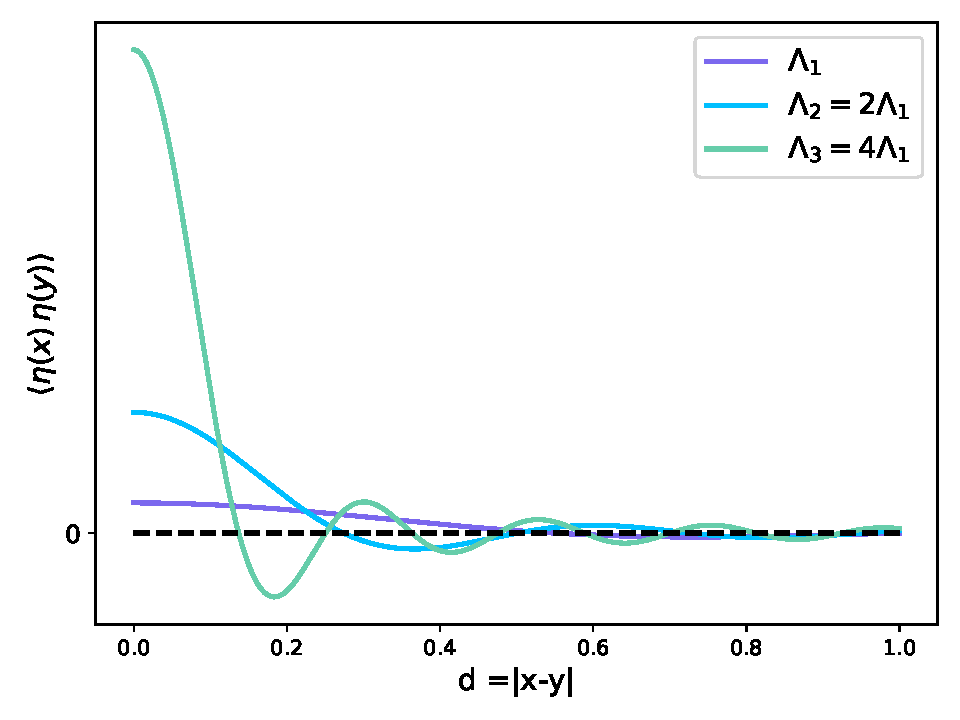
\includegraphics[scale=0.6]{figures/bessel.pdf}
    \caption[Correlated noise]{Noise correlation as a function of $d=|x-y|$ for three different values of the cutoff $\Lambda_1 < \Lambda_2 < \Lambda_3$, in arbitrary units. The plot is qualitative, but shows clearly that with a regulated noise, small-distance ($d \ll 1/\Lambda$) noise correlations are present, while the noise remains uncorrelated at large distances ($d \gg 1/\Lambda$), as in the white noise case.}
    \label{fig:bessel}
\end{figure}
\raggedright Another intuitive and interesting aspect of the dynamics in the presence of coloured noise can be deduce by looking at the field expression in terms of the retarded Langevin Green function \cite{Damgaard1987StochasticQuantization}, which is here not derived, but reported from \cite{Pawlowski2017CoolingNoise}
\begin{equation*}
        \phi(x, \tau) = \int_{x^{\prime}} \int_{-\infty}^\tau \mathrm{d} \tau^{\prime} G\left(x-x^{\prime}, \tau-\tau^{\prime}\right) \, \left[r_{\Lambda}\left(\Delta_x\right) \eta\left(x, \tau^{\prime}\right)-\frac{\delta S}{\delta \phi}|_{p=0} \, \phi\left(x^{\prime}, \tau\right)\right]
\end{equation*}
where
\begin{equation*}
    G\left(x-x^{\prime}, \tau-\tau^{\prime}\right) =\theta\left(\tau-\tau^{\prime}\right) \int_p \mathrm{e}^{-i p \cdot\left(x-x^{\prime}\right)} \mathrm{e}^{-\left(\tau-\tau^{\prime}\right)\left(p^2+m^2\right)}
\end{equation*}
By looking at the first term in the square bracket, one can conclude that there is no propagation of modes with momentum $p^2\geq \Lambda^2$ due to the noise term, but one can still have contribution from modes $p^2 > \Lambda^2$ from the second term, which corresponds to the deterministic part of the equations of motion. Stated differently, UV quantum fluctuations with $p^2 > \Lambda^2$ are removed from the dynamics of $\phi$, but still contribute classically. \\~\\
Generally speaking, the stationary distribution probability of the regulated stochastic process is given by \cite{Pawlowski2017CoolingNoise}
\begin{equation}
    \mathcal{P}_\Lambda(\phi) = \frac{1}{Z} \, \exp\left(-S_\Lambda[\phi]\right) = \frac{1}{Z} \, \exp\left(-(S[\phi] + \Delta S_\Lambda[\phi])\right)
    \label{eq:probability_field_configuration_regularised}
\end{equation}
where the correction term $\Delta S_\Lambda[\phi]$, for the specific case of the regulator \eqref{eq:regulator} reads
\begin{equation*}
        \Delta S_{\Lambda}[\phi]=\frac{1}{2} \int_p \phi_p \, \Lambda^2\left(\frac{1}{r_{\Lambda}\left(p^2\right)}-1\right) \, \phi_{-p}
\end{equation*}
\textcolor{red}{at this point mention that this is the stationary pdf that one gets with frg for sharp cutoff, and cite some papers.}

\section{Applications of coloured noise in lattice QFT}
\label{sec:lattice_with_coloured_noise}

\subsection*{Cooling and the continuum limit}
After the general introduction on coloured noise given in the previous paragraph, let us now look more closely on the lattice formulation and at some possible applications of the technique. \\~\\
To this end, let us consider a two-dimensional lattice with side lengths $L_t, L_x$ and spacing $a = a_x = a_t$. This implies a maximum momentum $p_\text{max} = \pi / a$ in each space-time direction and $N_x=L_x/a, N_t=L_t/a$ points in each direction. Let us also define 
\begin{equation}
	\Lambda^2 \equiv (p^x_\text{max})^2 + (p^t_\text{max})^2
\end{equation}
which indicates the maximum squared momentum on the given lattice. \\
We then consider a simulation with a regularised noise defined by a cutoff $\Lambda_\text{eff} \leq \Lambda$ and we define a dimensionless parameter
\begin{equation}
	s = \frac{\Lambda_\text{eff}}{\Lambda} \qquad 0 \leq s \leq 1
\end{equation}
Note that $\Lambda_\text{eff}$ implicitly defines a length scale given by  $a_\text{eff} = \pi/\Lambda_\text{eff}$.\\
Let us then consider a simulation with $s=1$ and a set of bare couplings $\{g^i_0\}$, and another simulation with $s'<1$ and new set of couplings $\{g^{i \, \prime}_0\}$. 
We now want to address the following question: is it possible to compensate the change in physical observables caused by the removal of the UV modes via regularised noise in the second simulation, by properly fine-tuning the bare parameters that enter the lattice discretised action? In other words, we want to encode the quantum fluctuations with $p^2 > \Lambda_\text{eff}^2$ in a redefitinion of the classical action so that the expectation value of the observables remains unchanged.\\
The issue is of course related to the renormalisation transformation introduced in chapter \ref{chap:background}. In particular we can exploit the connection between stochastic quantisation with coloured noise and the renormalisation group, as mentioned at the end of section \ref{sec:coloured_noise}, to accomplish the above mentioned goal. \\
As stated at the end of section \ref{sec:wilson_rg}, the Wilson RG flow of the dimensionless couplings and fields is dominated by the canonical scaling dimension of the corresponding dimensionful quantities, for high enough cutoff. 
We are interested in cooling the simulation by removing only the short-length fluctuations, hence we rely on this approximation as a lowest order Ansatz. This corresponds to a tree level RG rescaling. \\~\\
For what concerns the scalar part of the action, the rescaling at tree level is rather straightforward
\begin{equation*}
    \begin{aligned}
    \hat{m}_\phi^2 = (a^2m_\phi^2) \ \to \ s^2(a^2m_\phi^2) = s^2 \, \hat{m}_\phi^2, &\qquad \hat{\lambda} = (a^2\lambda) \ \to  \ s^2 (a^2\lambda) = s^2\hat{\lambda} \\
    \hat\phi = \phi \ &\to \ \phi = \hat\phi
    \end{aligned}
\end{equation*}
The fermionic part needs some more careful analysis. For simplicity, let us for the moment set $N_f = 1$. \\
In a lattice simulation one wants to perform the integral over the fermionic fields and works with the effective action \eqref{eq:effective_action_no_fermions}. In this case the drift is given by equation \eqref{eq:drift_continuum_full_theory}, with the fermionic contribution beeing
\begin{equation}
    	K_{\psi} = g \, \underset{s}{\tr}{D^{-1}}
	\label{eq:fermionic_drift_contribution}
\end{equation}
or, in terms of dimensionless quantities
\begin{equation*}
    \widehat{K}_{\psi} = (ag) \, \underset{s}{\tr}{(aD)^{-1}}
\end{equation*}
This implies that under a lattice block-spin transformation, where $a \to sa$,
\begin{equation}
    \widehat{K}_{\psi} \to  (sag) \, \underset{s}{\tr}{(saD)^{-1}} = \widehat{K}_{\psi}
    \label{eq:fermionic_rescaling_na\"ive}
\end{equation}
On the other side, when computing the drift via the original action \eqref{eq:full_action_continuum}, one gets (omitting $\tau$ and $x$ dependency)
\begin{equation}
    \begin{aligned}
        K(\tau, x) &= - \frac{\delta S}{\delta \phi(\tau, x)} = K_\phi - g \, \bar\psi\psi = \\
        &= -\left(-\partial^2_x + m_\phi^2\right) \phi - \frac{\lambda}{6} \, \phi^3 - g \, \bar\psi\psi
    \end{aligned}
    \label{eq:drift_continuum_from_full_action}
\end{equation}
where the fermionic contribution is given by
\begin{equation*}
    K_{\psi}' = - g \, \bar\psi\psi
\end{equation*}
Note that all the terms in the equation \eqref{eq:drift_continuum_from_full_action} have dimension 2, in units of energy, which means, in particular, that after a lattice block-spin transformation where $a \to sa$, one has
\begin{equation}
    \widehat{K}'_\psi = (ag) (a\bar\psi \psi) \to s^2 (ag) (a\bar\psi \psi) = s^2 \widehat{K}'_\psi
    \label{eq:rescaling_blinear}
\end{equation}
in contrast with \eqref{eq:fermionic_rescaling_na\"ive}. For this reason, in order to have the correct scaling, we compute the contribution to the drift without rescaling the Dirac operator (and hence the Yukawa coupling), and then rescale the whole drift via 
\begin{equation*}
    \widehat{K}_\psi \to s^2 \widehat{K}_\psi
\end{equation*}
so that the scaling dimension of the other terms in \eqref{eq:drift_continuum_from_full_action} is matched. \\~\\
We want to mention that this has important consequences on the issue of continuum limit of low-energy effective theories. In fact, in the standard lattice regularisation procedure, one always has $a \sim \Lambda^{-1}$, which means that the continuum limit $a \to 0$ is always connected to the limit $\Lambda \to \infty$, and this constitutes a problem for effective theories. The latters are in fact meant to be valid only up to a certain scale $\Lambda_\text{phys}$, hence one always needs $\Lambda \leq \Lambda_\text{phys}$. Cooling via coloured noise can provide a solution to this problem, since one can always keep the effective cutoff fixed at $\Lambda_\text{eff} = \Lambda_\text{phys}$, while taking the limits $a \to 0, \Lambda \to \infty$. 

\subsection*{Temperature control}
I have to wait for some results to see whether to include this or not :D